\documentclass{article}

\usepackage{times}
\usepackage{graphicx}
\usepackage{url} % for typesetting urls
\usepackage{color}
\usepackage{fancybox}
\usepackage{amssymb}
\usepackage{amsmath}
\usepackage{framed}
\usepackage[a4paper,lmargin=35mm,tmargin=35mm,bmargin=35mm,rmargin=35mm,twoside=false,marginpar=30mm]{geometry}

% ------------------------------------------------------------------------
\definecolor{lightgray}{RGB}{225,225,225}

\newenvironment{eg}{\par\noindent{\bf Example.}}{\hfill$\blacksquare$}
\newenvironment{insight}[1]{
\begin{framed}
\noindent\begin{minipage}[t]{0.05\textwidth}
{\Huge ?}
\end{minipage}%
\begin{minipage}[m]{0.95\textwidth}
{\bf #1}
}{\end{minipage}\end{framed}}

% ------------------------------------------------------------------------

\usepackage{listings}

% ==========================================
% Whiley LstListing Mode
% ==========================================

\pagestyle{plain}
\lstloadlanguages{Java}
\lstset{
        language=Java,
        keywords={function, method, type, assert, for, while, switch, is, if, case, return,
          else, process, define, as, requires, ensures, where, no,
          all, bool, int, byte, char, string, void, real, in, any, null
        },
        basicstyle=\small\ttfamily,
        commentstyle=\rmfamily\itshape,
        %%Uncomment the following line to avoid boldface keywords
        % keywordstyle=\ttfamily,
        stringstyle=\small\itshape,
        moredelim=*[s][commentstyle]{/*}{*/}, % allows keyword highlighting inside comments
        morecomment=[l][commentstyle]{//},      % single line comments are set by...
        backgroundcolor=\color{lightgray},
        frame=single, % adds a frame around the code
        frameround=tttt,
        framesep=0.25cm,
        texcl,                                                          % ...LaTeX
        moredelim=[is][\ttfamily]{<code>}{</code>}, % allows setting code inside multi-line comments
        moredelim=*[s][\ttfamily]{/*@}{*/}, % JML annotations
        moredelim=*[l][\ttfamily]{//@}, % JML annotations
        moredelim=**[is][\itshape]{/_}{_/}, % allows emphasizing sub-expressions
        moredelim=**[is][\bfseries]{/b_}{_b/}, % allows emphasizing sub-expressions
        escapeinside={(*@}{@*)}, %use (*@\label{line:desc}@*) to label lines for \ref
        mathescape=true,                % allow $ $ for math mode (will this break things?}
        tabsize=4,
	tab=\rightarrowfill,
        xleftmargin=1cm,
        xrightmargin=1cm,
        showspaces=false,
        showtabs=false,
        columns=fullflexible,
        numberstyle=\tiny,
        keepspaces=true,
        mathescape=true, % allows $ to switch in and out of math mode within listings
        literate={->}{{$\rightarrow$}}1 {<<}{{$\langle$}}1 {>>}{{$\rangle$}}1
           {tau}{{$\tau$}}1 {tau'}{{$\tau\prime$}}1 {(|}{{$\lpbar$}}1 {---}{{$\hole$}}1
           {-*-}{{$\times$}}1 {||_}{{$\lceilfloor$}}1 {_||}{{$\rceilfloor$}}1
           {/0}{{$\emptyset$}}1 {/bul}{{$\unit$}}1 {:->}{{$\mapsto$}}1
           {~}{$\sim$}1,
}


\title{\Huge Getting Started with Whiley}

\author{David J. Pearce}

\begin{document}
\maketitle
\begin{abstract}
  The aim of this document is to provide a short introduction to the
  Whiley programming language, in order to get you up and running
  quickly.  However, it is not intended to be a definitive reference.
  We'll walk through a number of simple examples illustrating the most
  interesting features of Whiley, and show you how to get it up and
  running.  We will be assuming some rudimentary knowledge of
  programming.
\end{abstract}
\tableofcontents
\clearpage
\section{Introduction}
The Whiley programming language has been in active development since
2009.  The language was designed specifically to help the programmer
eliminate bugs from his/her software.  The key feature is that Whiley
allows programmers to write {\em specifications} for their functions,
which are then checked by the compiler.  For example, here is the
specification for the \lstinline{max()} function which returns the
maximum of two integers:

\begin{lstlisting}
function max(int x, int y) => (int z)
// Must return either x or y
ensures x == z || y == z
// Return must be as large as x and y
ensures x <= z ${\tt \&\&}$ y <= z:
    ...
\end{lstlisting}
Here, we see our first piece of Whiley code.  This declares a function
called \lstinline{max} which accepts two integers \lstinline{x} and
\lstinline{y}, and returns an integer \lstinline{z}.  For now, we've
left out the body of this function and put ``\lstinline{...}'' in its
place.  The two \lstinline{requires} clauses form the function's {\em
  post-condition}, which is a guarantee made to any caller of this
function.  In this case, the \lstinline{max} function guarantees to
return one of the two parameters, and that the return will be as large
as both of them.  In plain English, this means it will return the
maximum of the two parameter values.  

When verification is enabled the Whiley compiler will check that every
function meets its specification.  For our \lstinline{max()} function,
this means it will check that body of the function guarantees to
return a value which meets the function's post-condition.  If not, the
compiler will report an error.  The advantage of supporting
specifications, is that they can help uncover bugs and other, more
serious, problems earlier in the development cycle.  This leads to
software which is both more reliable and more easily maintained (since
the specifications provide important documentation).

\subsection{Objectives}

Although the primary purpose of Whiley is to allow us to write
specifications on functions, we will not talk about that again until
the end of the document.  This goal of this article is to introduce
the core language without worrying too much about verification (since
this presents many challenges).  Indeed, it is only once we've
understood the basics of Whiley that we will will be ready to
investigate verification.

\subsection{Installation}

There are currently three ways to get setup with the Whiley
programming language:

\begin{itemize}
\item {\bf Web Browser.} By far the simplest way to get started with
  Whiley is by running it in your web browser (see
  Figure~\ref{whileyplay}).  Go to \url{http://whiley.org/play/} and
  you can get started straight away!
\item {\bf Eclipse Plugin.} If you're familiar with the Eclipse IDE or
  want to develop more serious programs in Whiley, then installing the
  Eclipse plugin is easy to do.  From within Eclipse, choose {\em
    Help$\rightarrow$Install New Software} from the menu.  Enter
  \url{http://whiley.org/eclipse} as the site, select the ``Whiley
  Eclipse Plugin'' and follow the on-screen instructions (see Figure~\ref{wyclipseinstall}).
\item {\bf Development Kit.} For those familiar with the command-line,
  installing the Whiley Development Kit (WDK) is another option.
  Furthermore, you'll be able to explore the source code for the
  Whiley system, and see how it all works!  To do this, visit
  \url{http://whiley.org/downloads/}.
\end{itemize}

More information of getting started with Whiley can be found at
\url{http://whiley.org/getting-started/}.  Finally, the Whiley system
is completely free and released under an open source license (BSD),
and you can get the latest code from \url{http://github.com/Whiley}.

\begin{figure}[!t]
\centering
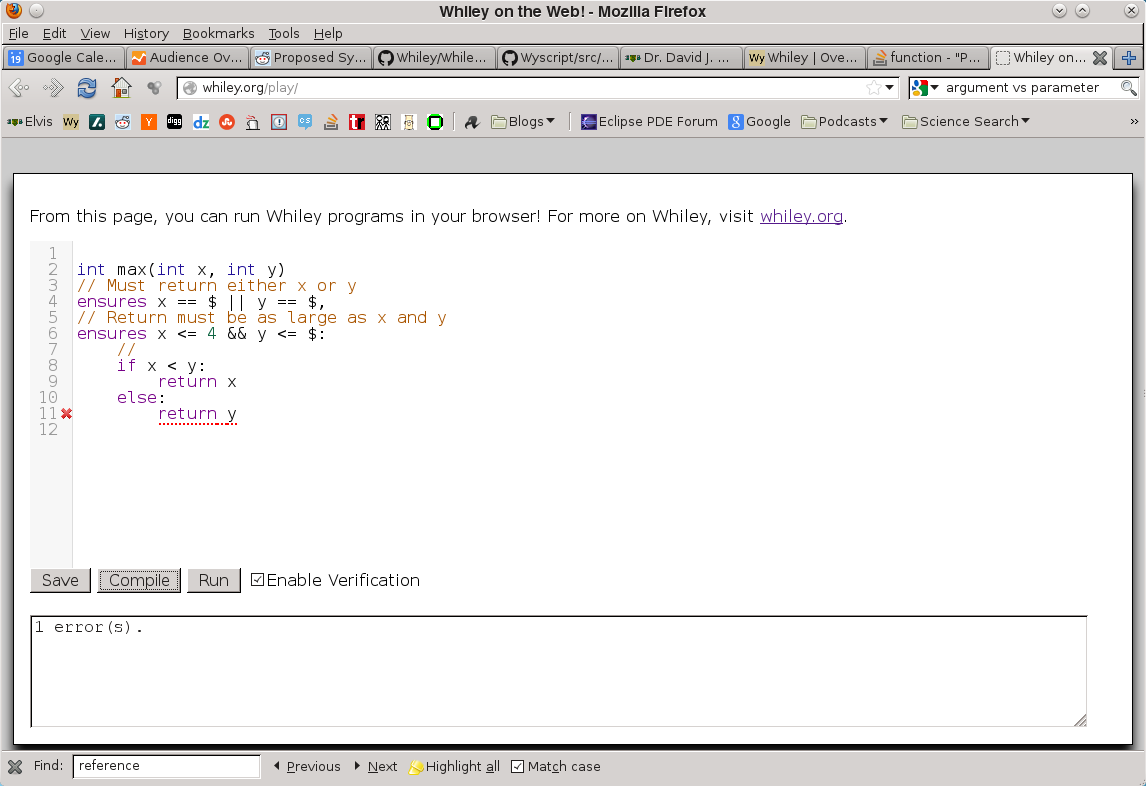
\includegraphics[width=0.9\textwidth]{../images/WhileyPlay.png}
\caption{Compiling a Whiley program using a web browser (Mozilla
  Firefox).  At the moment, the user's program is not correct since
  the system is reporting an error in red.}
\label{whileyplay}
\end{figure}

\begin{figure}[!t]
\centering
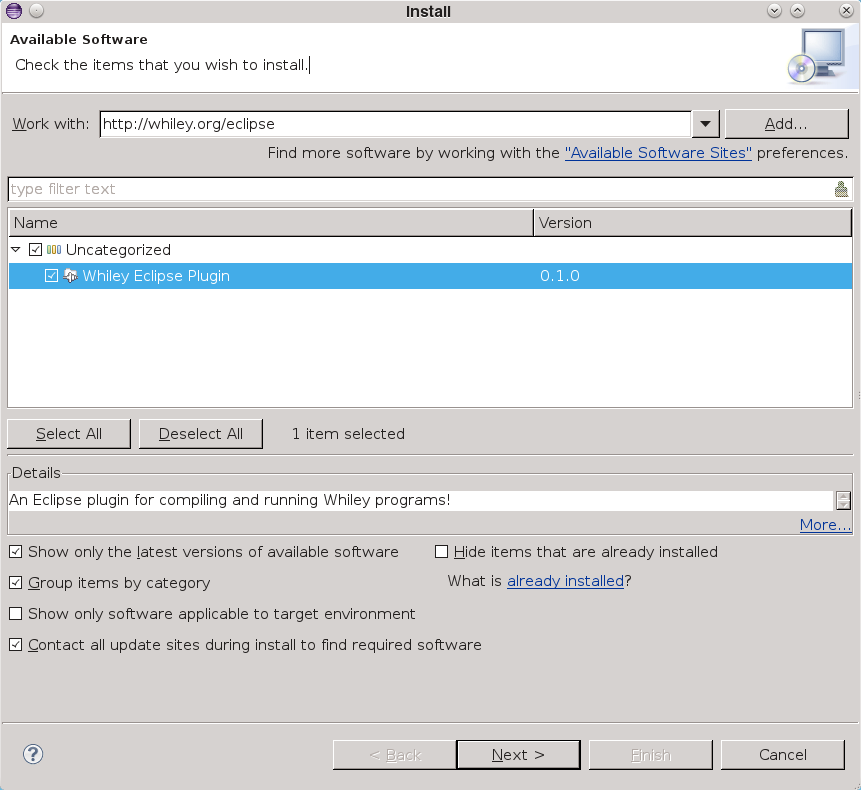
\includegraphics[width=0.9\textwidth]{../images/WyclipseInstallation.png}
\caption{Installing the Whiley Eclipse Plugin from within Eclipse.}
\label{wyclipseinstall}
\end{figure}

\clearpage

\newpage
\section{Quick Walkthrough}
This section provides a quick walk through of the main concepts and
ideas in the Whiley language.  Through a series of short examples,
we'll introduce the basic building blocks of the language.

\subsection{Booleans and Numbers}

As found in many languages, Whiley supports a range of primitive
datatypes for representing boolean, integers, real numbers, bytes,
characters, etc.  Of these, the most commonly used are:

\begin{itemize}
\item {\bf Booleans} are denoted by the type \lstinline{bool}.  This is the
  simplest of the primitive datatypes, and has only two possible
  values: \lstinline{true} or \lstinline{false}.
\item {\bf Integers} are denoted by the type \lstinline{int}.  Integers in
  Whiley are {\em unbounded}. This means that, in theory at least, a
  variable of type int can take on {\em any possible integer value};
  this differs from many other languages (e.g. Java), which limit the
  number of possible values (e.g. following 32-bit two's complement).
\item {\bf Real Numbers} are denoted by the type
  \lstinline{real}. Reals in Whiley are {\em unbounded
    rationals}. This means that, in theory at least, a variable of
  type real can take on {\em any possible rational value}. Again, this
  offers significantly better precision than, for example,
  \lstinline{float} or \lstinline{double} types based on IEEE754 as
  found in other languages (e.g. Java).
\end{itemize}


\noindent A very simple example which illustrates the \lstinline{int} and
\lstinline{bool} types is the following:
\begin{lstlisting}
function isLessThan(int x, int y) => bool:
    //
    if x < y:
        return true
    else:
        return false
\end{lstlisting}
This declares a simple function which returns \lstinline{true} if the
first parameter, \lstinline{x}, is less than the second,
\lstinline{y}, and \lstinline{false} otherwise.

\begin{insight}{Indentation Syntax.}
  From the above example you should notice that Whiley, unlike many
  languages, does not use curly braces (i.e. \verb+{ ... }+) to
  demarcate blocks of code.  Instead, Whiley uses {\em indentation
    syntax} which was popularised by the Python programming language.
  The start of a new code block is signalled by a preceding \verb+:+
  on the previous line.  The new block must be indented by at least
  one space (the actual amount doesn't matter) and all subsequent
  statements with the same indentation are included.
\end{insight}

\begin{insight}{Ints versus Reals.}
Unlike many other languages, Whiley provides a strong relationship
between values of type \lstinline{int} and those of type
\lstinline{real}.  Specifically, every \lstinline{int} value can be
represented precisely as a \lstinline{real} value.  Although it may
seem surprising, this is not true for many other languages
(e.g. Java), where there are \lstinline{int} (resp. \lstinline{long})
values which cannot be represented using \lstinline{float}
(resp. \lstinline{double})~\cite{GJSB05}.
\end{insight}

% \begin{lstlisting}
% function floor(real x) => int:
%     int num / int den = x    // extract numerator and denominator
%     int r = num / den        // integer division
%     if x < 0.0 && den != 1: 	 
%         return r - 1 
%     else:
%         return r 
% \end{lstlisting}

\subsection{Sets, Lists and Maps}

Like many modern programming languages, Whiley provides built-in types
for representing collections.  The following illustrates a short
function which multiplies a vector by a scalar:
\begin{lstlisting}
function vectorMultiply([real] vector, real scalar) => [real]:
    for i in 0 .. |vector|:
        vector[i] = vector[i] * scalar
    return vector
\end{lstlisting}
This illustrates a few of the common collection operations.  Firstly,
the size of a collection is obtained using the {\em length} operator
(i.e. \lstinline{|vector|} returns the length of \lstinline{vector}).
Secondly, the \lstinline{for} loop is useful for iterating over the
elements of a collection.  In this case, \lstinline{0 .. |vector|}
returns a {\em list} of consecutive integers from \lstinline{0} up to
(but not including) \lstinline{|vector|}.  Finally, the {\em list
  access} operator, \lstinline{vector[i]}, returns the element at
index \lstinline{i}.  The three different kinds of collections
supported in Whiley are:
\begin{itemize}
\item {\bf Sets} (e.g. \lstinline|{int}|) provide the simplest form of collection, and are constructing using a {\em set constructor} (e.g. \lstinline|{1,2,3}|).  They support the {\em set union} (e.g. \lstinline{xs + ys}), {\em set intersection} (e.g. \lstinline{xs & ys}) and {\em set difference} (e.g. \lstinline{xs - ys}) operators.  One can test for inclusion using the {\em element of} operator (e.g. \lstinline{x in xs}), or the {\em subset} (e.g. \lstinline{xs $\subset$ ys}) and {\em subset or equal} (e.g. \lstinline{xs $\subseteq$ ys}) operators.
  
\item {\bf Maps} (e.g. \lstinline|{int=>string}|) provide a halfway point between sets and lists.  They are similar to dictionaries in Python or the \lstinline{Map} interface in Java.  They can be viewed as a set of {\em key$\times$ value} pairs, where every key maps to exactly one value.  Maps are constructed using a {\em map constructor} (e.g. \lstinline|{1=>"hello",2=>"world"}|), and elements are accessed using the {\em map access} operator (e.g. \lstinline{map[i]}).  

\item {\bf Lists} (e.g. \lstinline{[int]}) are similar to arrays
  (e.g. in Java), but they can also be resized.  As can be seen above,
  they support the {\em list access} operator
  (e.g. \lstinline{vector[i]}).  They also support the {\em list
    append} operator (e.g. \lstinline{[1,2,3] ++ [4,5,6]}) and {\em
    sublist} operator (e.g. \lstinline{vector[0..2]}).  Finally, lists are constructed using a {\em list constructor} (e.g. \lstinline{[1,2,3]}).

\end{itemize}

All collection kinds can be iterated using the built-in
\lstinline{for} loop construct.  For example, here is a function to iterate a map looking for a particular value:

\begin{lstlisting}
// Return the set of all keys which map to a given value
function keysOf({int=>string} map, string value) => {string}:
    {string} result = {} // initialise result with empty set
    for k,v in map:      // loop over every key,value pair in map
        if v == value:
            result = result + {k} // add matching keys to result set
    // return result
    return result
\end{lstlisting}

\noindent This function iterates over each key$\times$value pair (i.e. \lstinline{k,v}) in a from integers to strings (i.e. \lstinline|{int=>string}|) using the \lstinline{for} statement.

\subsection{Records and Tuples}

\subsection{Strings and Characters}

\subsection{Value Semantics}
\label{value_semantics}
In Whiley, all compound structures (e.g. lists, sets, and records)
have {\em value semantics}.  This means they are passed and returned
by-value (as in Pascal, MATLAB or most functional languages).  But, unlike
functional languages (and like Pascal), values of compound types can
be updated in place.

Value semantics implies that updates to a variable only affects that
variable, and that information can only flow out of a function through
its return value.  Whiley has no general, mutable heap comparable to
those found in object-oriented languages.  Consider:
\begin{lstlisting}
 int f([int] xs):
     ys = xs
     xs[0] = 1
     ...
\end{lstlisting}
The semantics of Whiley dictate that, having assigned \lstinline{xs}
to \lstinline{ys} as above, the subsequent update to \lstinline{xs}
does not affect \lstinline{ys}.  Arguments are also passed by value,
hence \lstinline{xs} is updated inside \lstinline{f()} and this does
not affect \lstinline{f}'s caller.  That is, \lstinline{xs} is not a
{\em reference} to a list of \lstinline{int}; rather, it {\em is} a
list of \lstinline{int}s and assignments to it do not affect state
visible outside of \lstinline{f()}. 

Whilst this approach may seem inefficient, a variety of techniques
exist (e.g. reference counting) to ensure efficiency (see
e.g.~\cite{LH11,Shank01,Ode91}).  Indeed, the underlying
implementation does pass compound structures by reference and copies
them only when absolutely necessary.


\newpage
\section{Flexible Types}
The previous section introduced us to the basic types found in Whiley,
such as integers (\lstinline{int}), rationals (\lstinline{real}) and
booleans (\lstinline{bool}).  However, unlike many languages, Whiley
provides a flexible and powerful approach to typing which go well
beyond the basic forms.  In this section, we will examine this in more
detail.

\subsection{Flow Typing}
To improve the programmer experience and reduce unnecessary tedium,
Whiley employs a {\em flow typing} system.  What this means is that
the type of a variable can vary at different points within a function.
To make this work, Whiley employs {\em union types}~\cite{BC91,IN07} along with {\em variable retyping}.  The
following example illustrates how this works (where the body of
\lstinline{indexOf()} is left out for brevity):

\begin{lstlisting}
 function indexOf(string str, char c) => null|int:
    ...

 function split(string str, char c) => [string]:
    var idx = indexOf(str,c)
    // idx has type null$|$int
    if idx is int:
        // idx now has type int
        int below = str[0..idx]
        int above = str[idx..]
        return [below,above]
    else:
        // idx now has type null
        return [str] // no occurrence
\end{lstlisting}
Here, \lstinline{indexOf()} returns the first index of a character in
the string, or \lstinline{null} if there is none.  The type
\lstinline{null|int} is a {\em union type}, meaning it is either an
\lstinline{int} or \lstinline{null}.  The \lstinline{split()} function
splits a string into two pieces based on the first occurrence of a
given character \lstinline{c}, or leaves the string as is otherwise.
It calls \lstinline{indexOf()} to determine the first occurrence of
\lstinline{c} in \lstinline{str}.  Observe that variable
\lstinline{idx} has been declared as type \lstinline{var}, meaning the
compiler will automatically infer the best possible type for it.

In the above example, Whiley's flow typing system seamlessly ensures
that \lstinline{null} is never dereferenced.  This is because the type
\lstinline{null|int} cannot be treated as an \lstinline{int}.
Instead, one must first check it is an \lstinline{int} using a type
test, such as ``\lstinline{idx is int}''.  Whiley automatically
{\em retypes} \lstinline{idx} to \lstinline{int} when this is known to be
true, thereby avoiding any awkward and unnecessary syntax (e.g. a cast
as required in many languages).

\begin{insight}{Null References.}  In many languages (e.g. C/C++,
  Java, etc) the use of \lstinline{null} is a significant source of
  error (see e.g.~\cite{Hoa09}).  For example, in Java dereferencing
  the \lstinline{null} value gives rise to a
  \lstinline{NullPointerException}, which is regarded as the most
  common form of error in Java~\cite{XYZ}.  The issue is that, in such
  languages, one can treat {\em nullable} references as though they
  are {\em non-null} references~\cite{Pier02}.  In the research
  literature, there have been many proposals to solve this problem
  using static type systems
  (e.g.~\cite{PQVHV01,FL03,KH07,CFJJ06,CJ07,MPPD08,Hub08,HJP08}).
  Unfortunately, at the time of writing, very few languages have
  incorporated such ideas.
\end{insight}

\begin{insight}{Intersections and Negations.}
  Whiley also supports so-called {\em intersection} and {\em negation}
  types.  Whilst these can be expressed directly in source code, they
  are generally less useful than unions.
\end{insight}

\begin{insight}{Untagged Unions}.  Often confusion surrounding untagged
    versus tagged unions.  The latter are more common, and sometimes
    known as {\em sum types}.
\end{insight}

\subsection{Recursive Types}
To represent tree-like structures, Whiley provides {\em recursive
  types} which are similar to the algebraic data types found in
functional languages (e.g. Haskell, ML, etc).  For example:
\begin{lstlisting}
// A linked list is either the empty list or a link
type LinkedList is EmptyList | Link

// The empty list contains no links
type EmptyList is null

// A single link in a linked list
type Link is {int data, LinkedList next}

// Return the length of a linked list (i.e. the number of links it contains)
int length(LinkedList l):
  if l is null:    
    return 0 // l now has type null
  else:    
    return 1 + length(l.next) // l now has type \{int data, LinkedList next\}
\end{lstlisting}
Here, \lstinline{LinkedList} is a recursive type representing a linked
list (i.e. a sequence of zero or more links).  The empty list is
defined as \lstinline{null}, whilst each link contains a
\lstinline{data} field.  The type \lstinline{LinkedList} is defined in
terms of itself (i.e. it is recursive) and describes linked lists of
arbitrary size.

\begin{insight}{Value Semantics.}
  As discussed in \S\ref{value_semantics} all compounds structures in
  Whiley are passed by value, {\em including recursive types}.  This
  differs from common languages (e.g. Java), where linked structures
  are typically composed from {\em references} to link objects.  This
  means, for example, that linked structures in such languages can
  share substructures, leading to subtle and hard-to-find bugs.  In
  Whiley linked structures, such as \lstinline{LinkedList}, can never
  share substructure.
\end{insight}

The above example also serves as another illustration of flow typing
in Whiley.  More specifically, on the false branch of the type test
``\lstinline{l is null}'', variable \lstinline{l} is automatically
retyped to \lstinline+{int data, LinkedList next}+ --- thus ensuring
the subsequent dereference of \lstinline{l.next} is safe.  No casts
are required as would be needed for a conventional imperative language
(e.g. Java).  Finally, like all compound structures, the semantics of
Whiley dictates that recursive data types are passed by value (or, at
least, appear to be from the programmer's perspective).

%\subsection{Polymorphism \& Encapsulation}
%Two important hallmarks of the object-oriented paradigm are
%polymorphism and encapsulation.  The former is typically achieved
%through inheritance and/or interfaces, whilst the latter typically
%exploits \lstinline{public} / \lstinline{private} modifiers.  Whiley
%does not permit \lstinline{public} or \lstinline{private} modifiers in
%records.  Instead, Whiley employs a simple form of {\em existential
%type}~\cite{}, illustrated as follows:
%
%\begin{lstlisting}
% define Shape as { 
%   bool contains(int x, int y, Shape this), 
%   ... 
% }
%\end{lstlisting}
%This declares what is, essentially, an interface.  The
%``\lstinline{...}''  notation is significant here, as it denotes
%unknown --- or {\em existential} --- state~\cite{Cook09}.  We can then
%``implement'' this interface as follows:
%
%\begin{lstlisting}
% define Square as {
%   int x, int y, int width, int height,   
%   bool contains(int x, int y, Square this)
% }
%
% bool defSqContains(int x, int y, Square sq):
%     if x >= sq.x && x < (sq.x + sq.width):
%         return y >= sq.y && 
%                y < (sq.y + sq.height)
%     return false
%
% Square defSquare(int x, int y, int w, int h):
%     return {x: x, y: y, width: w, height: h,
%             contains: &defSqContains}
%\end{lstlisting}
%{\bf THIS NEEDS WORK --- IT'S BROKEN}

\subsection{Structural vs Nominal Types}
Statically typed languages, such as Java, employ {\em nominal typing}
for recursive data types.  This means that two otherwise identical
types with different names are considered distinct and, for example, a
variable of one type cannot flow into the other.  In contrast, Whiley employs {\em structural typing} of records~\cite{Card88} to give greater flexibility.  This means that the name of a type is, generally speaking, unimportant.  Instead, identical types (i.e. those with identical {\em structure}) with different names are still considered identical in Whiley.  For example:

\begin{lstlisting}
// Define the notion of a "rectangle"
type Rectangle is { int x, int y, int width, int height }
// Define the notion of a "bounding box"
type BoundingBox is { int x, int y, int width, int height }

// Define a function for computing the area of a rectangle
function area(Rectangle rect) => int:
    return rect.width * rect.height
\end{lstlisting}

In this example, the types \lstinline{Rectangle} and \lstinline{BoundingBox} are {\em identical} and can be used interchangeably.  For example, if we have a variable of type \lstinline{BoundingBox}, we can safely pass it to the \lstinline{area()} function above to compute its area.

\subsubsection{Nominal Types}

It is possible to simulate nominal types in Whiley.

\subsection{Subtyping}

An important concept in many modern programming languages is that of {\em subtyping}.  This defines a relationship between otherwise different types (i.e. which do not have identical structure).  

\subsection{Coercions}

A {\em coercion} converts a value of one type into a corresponding value of another type.  For example, in Whiley, we can coerce the \lstinline{int} value ``\lstinline{0}'' into the \lstinline{real} value ``\lstinline{0.0}''.  Many programming languages permit both {\em implicit} and {\em explicit} coercions, with the latter more commonly referred to as {\em casting}.  Implicit coercions occur without explicit direction from the programmer, and are often considered dangerous because of this.  

\begin{insight}{Lossless Coercions?}
The Java programming language attempts to enforce a requirement that implicit coercions are {\em lossless}.  Thus, any coercion which may result in a loss of information must be made explicit through the use of a cast.  Unfortunately, Java does permit implicit lossy coercions by, for example, allowing \lstinline{int} values to be implicitly coerced into \lstinline{float} values --- because not every \lstinline{int} value can be represented by a \lstinline{float} in Java.
\end{insight}

To address the issues surrounding implicit coercions, Whiley only permits implicit coercions which are lossless.  That is, which do not result in a loss of information.  In contrast, {\em lossy} coercions require an explicit cast be used to ``force'' the coercion.  The following example illustrates:
\begin{lstlisting}
type Link is {int data, LinkedList next}
type LinkedList is null | Link
type OrderedList is null | {
  int data, int order, OrderedList next
}
\end{lstlisting}
Here, we have defined a standard linked list and a specialised
``ordered'' list.  The intuition is that \lstinline{order < next.order} for each node in an \lstinline{OrderedList} (although the details of how this is done are unimportant here).   These two types are not considered identical because they have different structure (i.e. \lstinline{OrderedList} has an additional field, \lstinline{order}).  However, there is still a subtyping relationship between them (i.e. \lstinline{OrderedList} subtypes \lstinline{LinkedList}).  Thus, an instance of \lstinline{OrderedList} can be used where a \lstinline{LinkedList} was expected.  For example:

\begin{lstlisting}
function sum(LinkedList l) => int:
    if l is null:
        return 0
    else:
        return l.data + sum(l.next)
\end{lstlisting}

This defines a simple recursive function for computing the length of a \lstinline{LinkedList}.  Instances of \lstinline{OrderedList} can be passed into this function by {\em coercing} them to instances of \lstinline{LinkedList}:

\begin{lstlisting}
function sum(OrderedList l) => int:
    return sum((LinkedList) l)
\end{lstlisting}

Here, we have used an explicit coercion (i.e. a cast) from \lstinline{OrderedList} to \lstinline{LinkedList}.  This must be done explicitly because the coercion is lossy because the field \lstinline{order} is discarded during the coercion.

\begin{insight}{Lossless Coercions.}
Whiley (unlike Java) supports lossless coercion from \lstinline{int} values to \lstinline{real} values.  This is because arithmetic in Whiley is unbounded and, hence, every value of \lstinline{int} type has a corresponding value of \lstinline{real} type (though not vice-versa).
\end{insight}


\newpage
\section{Functional vs Imperative}



\subsection{Function Purity}
Much research has been done on functional purity for object-oriented
languages (e.g.~\cite{Pea11,Rou04,SR05,MRR02}), because it makes 
many things more tractable, including: {\em automatic
 parellelisation}~\cite{ABCR10,CRPAHBW10}, {\em software
 verification}~\cite{Leav02,BNSS04,BA05,DL07}, {\em query
 systems}~\cite{LHS97,WPN08}, {\em compiler
 optimisations}~\cite{Cla97,LLH05,ZRKW08} and more.

\subsection{Objects and References}
\subsection{Simulating Interfaces}
\newpage
\section{Example: Calculator}
\begin{figure}[!p]
\begin{lstlisting}[numbers=left]
 define Var as string
 define Op as { ADD, SUB, MUL, DIV }
 define BinOp as { Op op, Expr lhs, Expr rhs } 
 define ListAccess as { Expr lhs, Expr rhs } 

 define Value as int | [Value] | null

 define Expr as int | Var | BinOp | [Expr] | ListAccess 

 Value eval(Expr e, {Var->Value} env):
    if e is int:
        return e
    else if e is Var && e in env:
        // look up variable's value
        return env[e]
    else if e is BinOp:
        // evaluate left and right expressions
        lhs = eval(e.lhs,env)
        rhs = eval(e.rhs,env)
        // sanity check
        if !(lhs is int && rhs is int):
            return null // stuck
        // evaluate result
        switch e.op:
            case ADD:
                return lhs + rhs
            case SUB:
                return lhs - rhs
            case MUL:
                return lhs * rhs
            case DIV:
                if rhs != 0:
                    return lhs / rhs
    else if e is ListAccess:
        // evaluate src and index expressions
        src = eval(e.lhs,env)
        index = eval(e.rhs,env)
        // santity check
        if src is [Value] && index is int
           && index >= 0 && index < |src|:
            return src[index]
    else if e is [Expr]:
        lv = []
        // evaluate items in list constructor
        for i in e:
            v = eval(i,env)
            if v == null:
                return v
            else:
                lv = lv + [v]
        return lv
    // some kind of error occurred, so propagate upwards
    return null
\end{lstlisting}
\caption{Whiley code for a simple expression tree and evaluation
  function.  This makes extensive use of type tests, both for
  distinguishing expressions and error handling.  Flow-sensitive
  typing greatly simplifies the code, which would otherwise require
  numerous unnecessary casts.}
\label{eg1}
\end{figure}

Figure~\ref{eg1} provides a simple implementation of expressions,
along with code for evaluating them.  The types \lstinline{Expr} and
\lstinline{Value} are algebraic data types, with the latter defining
the set of allowed values.  Type \lstinline{Op} is an enumeration,
whilst \lstinline{BinOp} and \lstinline{ListAccess} are records which
form part of \lstinline{Expr}.  Parameter \lstinline{env} is a map
from variables to \lstinline{Values}.  Finally, \lstinline{null} is
used as an error condition to indicate a ``stuck'' state (i.e. the
evaluation cannot proceed).

The code in Figure~\ref{eg1} makes extensive use of runtime type tests
to distinguish different expression forms (e.g.  
``\lstinline{e is int}'').  These work in a similar fashion to Java's
\lstinline{instanceof} operator, with one important difference: they
operate in a flow-sensitive fashion and automatically {\em retype}
variables after the test.  As an example, consider the type test
``\lstinline{e is int}'' on Line 11.  On the true branch, variable
\lstinline{e} is automatically retyped to have type \lstinline{int}.
Likewise, on the false branch, \lstinline{e} is now known {\em not} to
have type \lstinline{int} (and any attempt to retest this yields a
compile-time error).

Figure~\ref{eg1} also employs runtime type tests to identify and
propagate errors.  For example, having evaluated the left- and
right-hand sides of a \lstinline{BinOp}, we check on Line 21 that both
are \lstinline{int} values (i.e. not list values or
\lstinline{null}).  After the check, Whiley's flow-sensitive type
system automatically retypes both \lstinline{lhs} and \lstinline{rhs}
to \lstinline{int}.  For \lstinline{ListAccess} expressions, we check
on Line~39 that \lstinline{src} is a list value, and that
\lstinline{index} is an \lstinline{int}.  The latter is achieved with
``\lstinline{index is int}''.  As \lstinline{src} is retyped within the
condition itself, the subsequent use of \lstinline{|src|} on Line~40
is type safe.

Implementing our expression language in a statically-typed language,
such as Java, would require code that was more cumbersome, and more verbose
than that of Figure~\ref{eg1}.  One reason for this is that, in
languages like Java, variables must be {\em explicitly} retyped after
\lstinline{instanceof} tests.  That is, we must insert casts to update
the types of tested variables and, since variables can have only one
type in Java, introduce temporary variables to hold these new types.
For example, after a test ``\lstinline{e instanceof BinOp}'' we must
introduce a new variable, say \lstinline{r}, with type
\lstinline{BinOp} and assign \lstinline{e} to \lstinline{r} using an
appropriate cast.  A Java implementation would also (most likely)
break up the test on Line 39, since it would otherwise need two
identical casts (one inside the condition for \lstinline{|src|}, and
one on the true branch for \lstinline{src[index]}).

In an object-oriented language, such as Java, a direct conversion of
Figure~\ref{eg1} might not be optimal.  Instead, the {\em visitor
  pattern}~\cite{gofbook} can be used to distinguish different
expression forms.  Using the visitor pattern reduces the amount of
explicit retyping required.  This is because the different expression
forms are explicitly given as parameters to the visitor methods.
However, using the visitor pattern is a heavyweight solution which is
not suitable in all situations.  In particular, it would not eliminate
all forms of explicit retyping from Figure~\ref{eg1}.  In this case,
explicit variable retyping will still be required to properly handle
the different values returned from \lstinline{eval()}.  For example,
to check \lstinline{BinOp}s are evaluated on \lstinline{int} operands
(Line~21), and that \lstinline{src} gives a list and \lstinline{index}
an \lstinline{int} (Line~39).

%% Functional programming languages provide {\em pattern matching} to
%% distinguish different forms of algebraic data type~\cite{duny}.  Like
%% the visitor pattern, this can be used to reduce the amount of explicit
%% retyping that is required.  {\bf [WHAT ELSE TO SAY HERE?]}


\paragraph{Code Reuse.}
Whiley's flow type system can expose greater opportunities
for code reuse:
\begin{lstlisting}[numbers=left]
{string} usedVariables(Expr e):
    if e is Var:
        return {e}
    else if e is BinOp || e is ListAccess:
        l = useVariables(e.lhs)
        r = useVariables(e.rhs)
        return l + r  // set union
    else if e is [Expr]:
        ...
    else:
        return {}
\end{lstlisting}

On Line 5, variable \lstinline{e} has type
\lstinline{BinOp|ListAcccess}.  The use of \lstinline{e.lhs} at this
point is type safe, since we can perform operations common to all
types of a union and, in particular, unions of records expose common
fields (similar to a {\em common initial sequence} for
\lstinline{union}s of \lstinline{struct}s in
C~\cite[\S6.3.2.3]{ISO90}).

In languages like Java, exploiting code reuse in this way requires
careful planning, as common types must be explicitly related in the
class hierarchy.  In contrast, Whiley's flow-sensitive type system
lets us exploit opportunities for code reuse in an ad-hoc fashion, as
and when they occur.



\subsection{Objective Objects}
%% \subsection{Processes}
%% As discussed already, Whiley adopts the Actor model of concurrency.
%% Here, processes --- or {\em actors} --- communicate via message
%% passing.  In Whiley, messages are processed using {\em methods} which,
%% unlike functions, may have side-effects.  The following illustrates a
%% simple example:
%% \begin{lstlisting}
%%  define Queue as process { [Packet] pkts }

%%  Packet Queue::get():
%%      pkt = items[0]
%%      this->pkts = pkts[1:]
%%      return pkt

%%   void Queue::put(Packet pkt):
%%       this->pkts = pkts + [pkt]
%%  \end{lstlisting}
%% Instances of \lstinline{Queue} are processes containing lists of
%% \lstinline{Packet}s.  Two methods, \lstinline{get()} and
%% \lstinline{put()}, are provided for manipulating them.  Methods are
%% distinguished from functions in Whiley by the \lstinline{R::m()}
%% syntax, where \lstinline{R} is the type of the receiver, and
%% \lstinline{m} the message name.  Furthermore, methods with
%% \lstinline{void} return type are {\em asynchronous}, whilst those
%% producing a value are {\em synchronous}.  

%% The semantics of processes dictates that each invocation of
%% \lstinline{get()} or \lstinline{put()} is processed atomically.  That
%% is, we cannot have two invocations of these methods executing
%% simultaneously.  Thus, there is no need to explicitly synchronise on
%% the field \lstinline{pkts}, as it can never be modified concurrently.
%% % %{\bf [BROADCASTING, ERROR HANDLING]}


\newpage
\section{Verification}

As discussed in the introduction, an important feature of Whiley is
{\em verification}.  That is made up of two aspects: firstly, the
ability to write specifications for functions and methods in Whiley;
secondly, the ability of the compiler to check the body of a function
or method meets its specification.

Unfortunately, specifications is not always straightforward and
requires considerable attention to detail.  Nevertheless, with
practice, it can easily fit into the routine of day-to-day
development.  In this section, we'll explore the basics of
verification in Whiley using some small examples.  In the following
section, we'll look at a larger and more example.

\subsection{Loop Invariants}

To complete our implementation of the \lstinline{indexOf()} function,
we need to add some hints to help the Whiley compiler.  These are
called {\em loop invariants}.  A loop invariant is a property which
holds before and after each iteration of the loop.  There are three
key points about loop invariants:
\begin{enumerate}
\item The loop invariant must hold on entry to the loop.
\item Assuming the loop invariant holds at the start of the loop body
  (along with the condition), it must hold at the end.
\item The loop invariant (along with the negated condition) can be
  assumed to hold immediately after the loop.
\end{enumerate}

To illustrate these three aspects, we'll use some simple loop
examples.  For example, consider the following example:

\begin{lstlisting}
function f(int x) => (int y)
// return cannot be negative
ensures y >= 0:
    //
    i = 0
    while i < x where i > 0:
        i = i + 1 
    //
    return i
\end{lstlisting}

Loop invariants in Whiley are indicated by the \lstinline{where}
clause.  Thus, in the above example, the loop invariant is
``\lstinline{i > 0}''.  Compiling the above program with verification
enabled will fail with an error.   This is because the loop invariant
does not hold on entry to the loop (item 1 above).
\newpage
\section{Example: IndexOf Function}

To better illustrate verification in Whiley, we'll consider specifying a simple function.  This is the \lstinline{contains()} function, described as follows:

\begin{lstlisting}
// Return the lowest index in the items list which equals the given item.
// If no such index exists, return null.
function indexOf([int] items, int item) => int|null:
    ...
\end{lstlisting}

This is a common function found in the standard libraries of many
programming languages.  The body of the function examines each element
of the \lstinline{items} list and check whether or not it equals
\lstinline{item}.  To start with, we won't worry too much about the
body of the \lstinline{indexOf()} function.  Instead, we'll
progressively build up the specification until we are happy with it.
Then, we'll give an implementation of the function which meets this
specification.\\

\noindent To specify this function, we want to ensure three properties:

\begin{enumerate}
\item If the return is an integer \lstinline{i}, then
  \lstinline{items[i] == item}.
\item If the return is \lstinline{null}, there is no index
  \lstinline{j} where \lstinline{items[j] == item}.
\item If the return is an integer \lstinline{i}, then there is
  no index \lstinline{j} where \lstinline{j < i} and
  \lstinline{items[j] == item}.
\end{enumerate}

These properties determine how a correct implementation of the
\lstinline{indexOf()} function should behave.  We refer to them as the
{\em specification} of the \lstinline{indexOf()} function.

\subsection{Specifying Property 1 --- Return Valid Index}

The first of the above properties is the easiest, so lets start by
specifying that in Whiley.  At the same time, we'll also give an
initial implementation which satisfies this partial specification:

\begin{lstlisting}
function indexOf([int] items, int item) => (int|null r)
// If return value is an int i, then items[i] == item
ensures i is int ==> items[i] == item:
    //
    if |items| > 0 && items[0] == item:
        return 0
    else:
        return null
\end{lstlisting}

Here, we can see property (1) above written as an \lstinline{ensures}
clause in Whiley.  In particular, the phrase ``the return value is an
integer'' is translated into the condition ``\lstinline{i is int}''.
Likewise, the implication operator (i.e. \lstinline{==>}) is used to
say ``If ... then ...''.  We've also given an initial implementation
for the \lstinline{indexOf()} function which simply checks whether or
not \lstinline{items[0] == item}.  This implementation meets the
specification we have so far although, obviously, this is an
incomplete implementation of the \lstinline{indexOf} function!

\subsection{Specifying Property 2 --- Return Null if No Match}
Property (2) from our list above is more difficult to specify, because
it requires {\em quantification}.  There are several quantifiers
available in Whiley, including: \lstinline{all}, which allows us to
say ``for all elements in a list something is true''; and
\lstinline{no}, which allows us to say ``there is no element in the list
where something is true''. 

In Whiley, we can express property (2) from above in several different
ways.  The most direct translation would be:

\begin{lstlisting}
...
// If return is null, there is no index j where items[j] == item
ensures i is null ==> no { j in 0..|items| | items[j] == item }:
    ...
\end{lstlisting}

\noindent Here, the expression \lstinline{|items|} gives the length of
the items list, whilst the range expression \lstinline{0..|items|}
returns a list of consecutive integers from \lstinline{0} up to, but
not including, \lstinline{|items|}.  Instead of using the
\lstinline{no} quantifier, we could have equally used the
\lstinline{all} quantifier, like so:

\begin{lstlisting}
...
// If return is null, there is no index j where items[j] == item
ensures i is null ==> all { j in 0..|items| | items[j] != item }:
    ...
\end{lstlisting}

The above, however, is perhaps not as clear as the first translation.
Finally we can, in this case, avoid talking about indices altogether
like so:

\begin{lstlisting}
...
// If return is null, there is no index j where items[j] == item
ensures i is null ==> no { x in items | x == item }:
    ...
\end{lstlisting}

The above simple says ``there is no element \lstinline{x} in
\lstinline{items} where \lstinline{x == item}''.  Although this is
also not the most direct translation of the original property, it is a
rather convenient translation which achieves the same thing.

\subsection{Specifying Property 3 --- Return Least Index}
\subsection{Working Implementation}

At this point, we can now give the complete specification for the
\lstinline{indexOf()} function, along with an initial implementation:

\begin{lstlisting}
function indexOf([int] items, int item) => (int|null i)
// If return is an int r, then items[r] == item
ensures i is int ==> items[i] == item
// If return is null, then no element x in items where x == item
ensures i is null ==> no { x in items | x == item }
// If return is an int i, then no index j where j $<$ i and items[j] == item
ensures i is int ==> no { j in 0 .. i | items[j] == item }:
    //
    i = 0
    while i < |items|:
       if items[i] == item:
           return i 
       i = i + 1
    //
    return null
\end{lstlisting}

The implementation of \lstinline{indexOf()} given above meets the
function's specification.  Unfortunately, whilst this is true, the
Whiley compiler needs help to determine this.  Figure~\ref{eg_indexOf}
illustrates what happens when we compile the above code with
verification enabled.

\begin{figure}[!t]
\centering
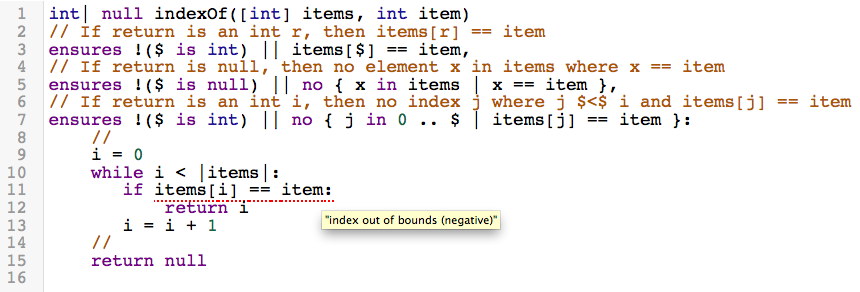
\includegraphics[width=1.0\textwidth]{../images/indexOf.png}
\caption{Illustrating our first working version of the
  \lstinline{indexOf} function being compiled with verification
  enabled.  The compiler is reporting an error stating ``{\em index out of
  bounds (negative)}''.  This is because the compiler believes
  \lstinline{i} may be negative at this point.  Although we know this
  is not true, we must write a {\em loop invariant} to help the
  compiler see this.}
\label{eg_indexOf}
\end{figure}

\subsection{Verified Implementation}
Although our implementation of \lstinline{indexOf()} given above is
correct, it currently does not verify.  Although this distinction may
seem unimportant, it goes to the heart of what verification is about.
That is, we know the implementation of \lstinline{indexOf()} is
correct because we, {\em as humans}, have looked at it and believe it
is.  Whilst may be a reasonable approach for small examples, it
certainly is not for larger and more complex programs.  Humans are
fallible and we can easily believe something is true when it is not.
Therefore, we want a mechanical system which can examine a program and
report ``{\em Yes, I agree that this is correct}''.  Whiley provides
such a system when verification is enabled.  

Unfortunately, Whiley is not as smart as a human and often there will
be things we know that it does not.  In such cases, we need to help
Whiley by adding hints into our programs.  In this case, we need to
add some loop invariants (recall \S\ref{loop_invariants}) to help
Whiley verify our implementation of \lstinline{indexOf()}.  The first
part of the loop invariant we need is straightforward.  Since
\lstinline{i} is modified in the loop, we need am invariant to ensure
\lstinline{i >= 0} when \lstinline{items[i]} is accessed:

\begin{lstlisting}
    ...
    i = 0
    while i < |items| where i >= 0:
        ...
        i = i + 1    
\end{lstlisting}
We can see that this invariant holds on entry to the loop (i.e. since
\lstinline{i = 0} on entry).  Furthermore, if \lstinline{i >= 0} then \lstinline{i+1 >= 0} follows and, hence, the loop
invariant holds after each iteration.

\newpage
\section{Example: Microwave Oven}
\begin{figure}[!t]
\centering
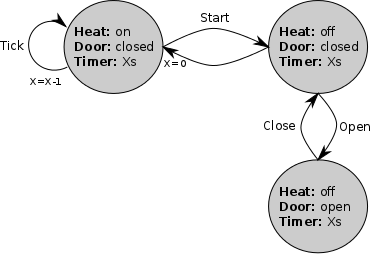
\includegraphics[width=0.75\textwidth]{../images/microwave.png}
\caption{A state-machine diagram for the microwave oven}
\end{figure}


\appendix
\section{Foreign Function Interface}
\label{s_ffi}
\section{Verification Conditions}
Talk about how to generate and see verification conditions.
\bibliographystyle{unsrt}
\bibliography{abbrevs,references}

\end{document}
